The analysis of massive datasets has become a necessary component of virtually all technical fields, as well as the social and humanistic sciences, in recent years. Given that rapid improvements in sensing and processing hardware have gone hand in hand with the data explosion, it is unsurprising that software for the generation and interpretation of this data has also attained a new frontier in complexity. In particular, simulation procedures such as Monte Carlo (MC) event generation can perform physics predictions even for theoretical regimes which are not analytically soluble. The bottleneck for such procedures, as is often the case, lies in the computational time and power which they necessitate.

Surrogate models, or metamodels, can resolve this limitation by replacing a resource-expensive procedure with a much cheaper approximation \cite{Sondergaard2003}. They are especially useful in applications where numerous evaluations of an expensive procedure are required over the same or similar domains, e.g. in the parameter optimisation of a theoretical model. The term "metamodel" proves especially meaningful in this case, when the surrogate model approximates a computational process which is itself a model for a (perhaps unknown) physical process \cite{Myers2002}. There exists a spectrum between "physical" surrogates which are constructed with some contextual knowledge in hand, and "empirical" surrogates which are derived purely from the underlying expensive model. 

In this internship project, in coordination with the UK Atomic Energy Authority (UKAEA) and Culham Centre for Fusion Energy (CCFE), we sought to develop a surrogate model for the tritium breeding ratio (TBR) in a Tokamak nuclear fusion reactor. Our expensive model was a MC-based neutronics simulation \cite{JonathanCollab}, itself a spherical approximation of the Joint European Torus (JET) at CCFE, which returns a prediction of the TBR for a given reactor configuration. We took an empirical approach to the construction of this surrogate, and no results described here are explicitly dependent on prior physics knowledge.

For the remainder of Section 1, we will define the TBR and set the context of this work within the goals of the UKAEA and CCFE. In Section 2 we will describe our datasets generated from the expensive model for training and validation purposes, and the dimensionality reduction methods employed to develop our understanding of the parameter domain. In Section 3 we will present our methodologies for the comparison testing of a wide variety of surrogate modelling techniques, as well as a novel adaptive sampling procedure suited to this application. After delivering the results of these approaches in Section 4, we will give our final conclusions and recommendations for further work.

\subsection{Problem Description}
\label{sec:problemdescription}

Nuclear fusion technology relies on the production and containment of an
extremely hot and dense plasma. In this environment, by design similar to that
of a star, hydrogen atoms attain energies sufficient to overcome their usual
electrostatic repulsion and fuse to form helium \cite{Hernandez2018}. Early prototype reactors
made use of the deuterium (\isotope[2]{H}, or \isotope{D}) isotope of hydrogen in order to
achieve fusion under more accessible conditions, but lead to limited success.
The current frontier generation of fusion reactors, such as JET and the
under-construction International Thermonuclear Experimental Reactor (ITER), make
use of tritium (\isotope[3]{H}, or \isotope{T}) fuel for further efficiency gain.
Experimentation at JET dating back to 1997 \cite{Keilhacker1999} has made significant headway in
validating deuterium-tritium (D-T) operations and constraining the technology
which will be employed in ITER in a scaled up form.

However, tritium is much less readily available as a fuel source than deuterium.
While at least one deuterium atom occurs for every \num{5000} molecules of
naturally-sourced water, and may be easily distilled, tritium is extremely rare
in nature. It may be produced indirectly through irradiation of heavy water
(\ce{D2O}) during nuclear fission, but only at very low rates which could
never sustain industrial-scale fusion power.

Instead, modern D-T reactors rely on tritium breeding blankets, specialised
layers of material which partially line the reactor and produce tritium upon
neutron bombardment, e.g. by 
\begin{align}
	\isotope[1][0]{n} + \hspace{3pt} \isotope[6][3]{Li} 
	&\longrightarrow \hspace{3pt} 
	\isotope[3][1]{T} + \hspace{3pt}\isotope[4][2]{He} \\
	\isotope[1][0]{n} + \hspace{3pt} \isotope[7][3]{Li} 
	&\longrightarrow \hspace{3pt} 
	\isotope[3][1]{T} + \hspace{3pt} \isotope[4][2]{He} + \hspace{3pt} \isotope[1][0]{n}
\end{align}
\begin{wrapfigure}{r}{0.45\textwidth}
  \vspace{-20pt}
  \begin{center}
    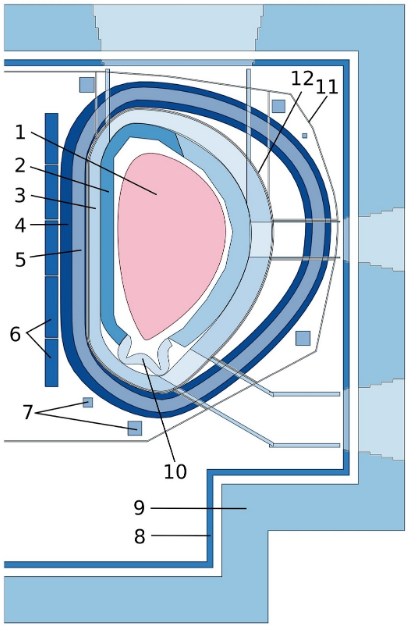
\includegraphics[width=0.48\textwidth]{fig1_tokamakdiagram.png}
  \end{center}
  \caption{Typical single-null reactor configuration as specified by BLUEPRINT \cite{Coleman2019}: 1 — plasma,
2 — breeding blankets }
\label{fig:tokamak}
\end{wrapfigure}
where T represents tritium and \isotope[7]{Li}, \isotope[6]{Li} are the more and
less frequently occurring isotopes of lithium, respectively. \isotope[6]{Li} has
the greatest tritium breeding cross-section of all tested isotopes \cite{Hernandez2018}, but due
to magnetohydrodynamic instability of liquid lithium in the reactor environment,
a variety of solid lithium compounds are preferred.

The TBR is defined as the ratio between tritium generation in the breeding
blanket per unit time and tritium fuel consumption in the reactor. The MC
neutronics simulations previously mentioned therefore must account for both the
internal plasma dynamics of the fusion reactor and the resultant interactions of
neutrons with breeding blanket materials. Neutron paths are traced through a CAD
model (e.g.~\cref{fig:tokamak}) of a reactor with modifiable geometry.

The input parameters of the computationally-expensive TBR model therefore fall
into two classes. Continuous parameters, including material thicknesses and
packing ratios, describe the geometry of a given reactor configuration. Discrete
categorical parameters further specify all relevant material sections, including
coolants, armours, and neutron multipliers. One notable exception is the
enrichment ratio, a continuous parameter denoting the presence of
\isotope[6]{Li}. Our challenge, put simply, was to produce a TBR function which
takes these same input parameters and approximates the MC TBR model with the
greatest achievable accuracy.

